\documentclass[twocolumn]{article}
\usepackage{hyperref}
\usepackage{graphicx}
\usepackage{caption}
\usepackage{subcaption}


\begin{document}
\onecolumn
\title{The Simulation of Real-Time Tasks on Non-Preemptive EDF Scheduling in Cloud Computing}
\author{TianZhang He\\ email: \href{mailto:hetianzhang91@gmail.com}{hetianzhang91@gmail.com}}
\date{September 15, 2017}
\maketitle

\section{Introduction}

\section{CloudSim}
CloudSim is a powerful and free source cloud computing simulation platform. However, there are few resources and on-line tutorials talking about how to simulate the run-time workloads with different submission time and deadline. In order to send the tasks dynamically to the specific Vm and decide the order in that VM queue the task will be inserted, we need to extend the Cloudlet, ResCloudlet, DataCenter Class, and implement a new DatacenterBroker and CloudletScheduler Class. In the extension version of the CloudSim, a new broker is implemented for run-time tasks and VM scheduling. Furthermore, a real-time task set is simulated in a non-preemptive Earliest Deadline First (EDF) algorithm for VM task scheduler with the new datacenter broker.

\subsection{CloudSim Extension}
\emph{[Talk about how to implement the run-time cloudlet submitting based on its submission time. CloudSim: SimEntity, SimEvent, defer and future queue.]}

\subsection{Broker and Task Scheduler}
The specific implementation in a new datacenter broker and a non-preemptive EDF task scheduler for cloudlets in the Vm.

Basically, the datacenter broker takes charge in sending the new tasks(cloudlets) to a specific Vm (a new or exist one) and destroy the idle Vm when receiving a cloudlet-return type SimEvent. Therefore, several SimEvent Tag should be used to implement the functions of a datacetner broker:

Meanwhile, the cloudlet scheduler deals with the task scheduling in one VM machine. Therefore, a new cloudlet scheduler (CloudletSchedulerEDF) is also developed by extending the CloudletSchedulerSpaceShared Class.

\section{Experiments and Evaluation}
Comparing the results of the processing based on time sharing task scheduling and non-preemptive EDF task scheduling algorithm by using the same workload on Cloudsim.
Amazon EC2 on-demand pricing:\\ 

\begin{tabular}{c|ccccc}
	\hline
General purpose & vCPU & ECU & Memory (GiB) & Instance Storage(GB) &Linux/UNIX Usage\\
\hline
m3.medium & 1 & 3 & 3.75 & 1*4 SSD & \$0.093 per Hour\\
\hline
\end{tabular}\\

the total execution time of the whole workload:
\begin{center}
\begin{tabular}{c|ccc}
	\hline
	Scheduler & Total Response Time & Created Vm &Total Vm running\\ \hline
	NP-EDF & 2936283.51 & 321 &2936292.41\\ \hline
	TimeShare & 3294489.6 & 103 & 2936296.7\\ \hline
\end{tabular}
\end{center}

Figure 1 shows the Histogram of 517 tasks' response time:\\
\begin{figure*}[htp]
\centering
\begin{subfigure}{0.5\textwidth}
	\centering
	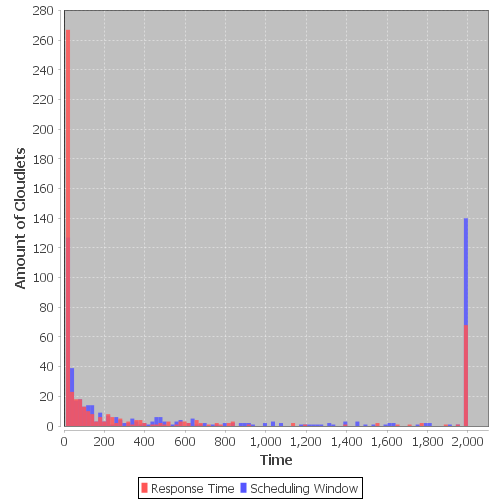
\includegraphics[width=8cm]{timesharedtaskHistogram}
	\caption{}
\end{subfigure}%
\begin{subfigure}{0.5\textwidth}
	\centering
	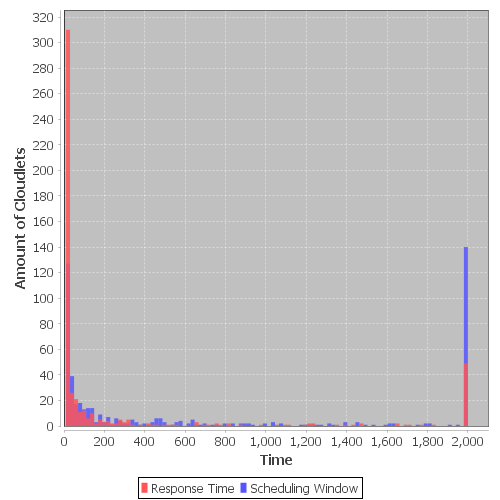
\includegraphics[width=8cm]{npedftaskHistogram}
	\caption{}
\end{subfigure}
\caption{(a): Time Sharing (b): NP-EDF}
\label{fig:taskhistogram}
\end{figure*}





\end{document}